\documentclass[conference]{IEEEtran}
% Packages
%\pdfobjcompresslevel=0
\usepackage{titlesec}
\usepackage{graphicx}
\usepackage[style=numeric, backend=biber, sorting=none,
            url=false, doi=false, isbn=false, eprint=false]{biblatex}
\addbibresource{Communication.bib}
\usepackage{algorithm}
\usepackage{algpseudocode}
\usepackage{booktabs}
\usepackage{float}
\usepackage{multirow}
\usepackage{enumitem}
\setlist[itemize]{leftmargin=*, itemsep=2pt}

% Title page
\title{Swarm Dialogues: Communication policies that Shape Embedded Evolution in ESP32 Collectives}
\author{Luis Yallico Ylquimiche}
\date{\today}

\begin{document}

% Title page
\maketitle
%add page numbers
\pagestyle{plain}

% Abstract
\begin{abstract}
We contribute a hardware-in-the-loop swarm that enables peer-to-peer ESP-NOW transmissions and quantifies the impact of communication policies in ESP32 swarms (3-13 robots). We compare stochastic peer ordering with link-aware scheduling and test two contention controls: per-agent message budgets and latency-bounded random micro-delays. Link-aware scheduling lowers latency and jitter by X\%, stochastic ordering spreads information faster by Y\% but increases collision errors by Z\% as density rises. Micro-delays stabilize latency with minimal throughput cost. Design rule: use stochastic scheduling with micro-delays for rapid diffusion, use link-aware scheduling when latency/jitter robustness is a priority.
\end{abstract}


\section{Introduction}

This study profiles swarm communication on ESP32 hardware and demonstrates how agent density, locomotion, topology inference, imposed message budgets, and stochastic transmission policies shape both network quality of service ($QoS$) and embedded evolution performance. Focusing on direct peer-to-peer links, we contribute with an empirical mapping that probes communication bottlenecks flagged in recent surveys, and evidence for extracting tangible design rules for swarm networks. \\

Swarm engineers draw inspiration from social biological systems such as ants, bees or termites to build decentralised robot collectives that are inherently robust to failure, flexible across tasks and scalable in number \cite{hamann_swarm_2018}. In swarm systems, collective intelligence emerges when individual robots trade packets of information among neighbouring robots. Classic ant-colony-optimisation work in the early 2000s has already proven that an indirect information exchange of "virtual-pheromones" can lead to agents collectively discovering optimal routing formations \cite{dorigo_ant_2000}. Hence, communication design is a first-order determinant of emergent behavior in swarms. \\

While coordination and task allocation have been widely studied in swarm robotics, two recent surveys agree that communication bandwidth, latency and energy usage are the main blockers to real-world swarm deployments \cite{ding_advancements_2023}\cite{an_multi-robot_2023}. These issues become more pronounced as swarms sizes scale, resulting in an increase in data volumes being transmitted among peers, often overwhelming individual agents' limited compute capabilities. Beyond sheer capacity, the architecture of the communication also matters. Many swarms rely on blind broadcast communication schemes that scale poorly, with collision rates rising sharply beyond a few dozen peers which tend to reduce the reliability of the network \cite{an_multi-robot_2023}. \\

Communication is equally critical when controllers evolve on-line. Recent embodied evolution studies explain that less communication can enhance swarm performance, as trimming neighbourhood size helps populations forget outdated beliefs and re-adapt faster \cite{hiraga_when_2023}\cite{ding_advancements_2023}. While our context is controller evolution, we instantiate it as a distributed global optimisation problem. Fixing behaviours and evolving solutions to a known objective, isolates the communication effects and makes adaptation dynamics comparable across conditions. \\

To support our investigation, we implement a hardware-in-the-loop framework by leveraging over-the-air (OTA) updates. For embedded evolution we use ESP-NOW with an island-model genetic algorithm (GA). Moving beyond simulation-heavy work, we experiment with Pololu 3Pi+ robots, as shown in Fig. \ref{fig:arena}b, and adopt a state-of-the-art cloud enabled system that captures granular packet and evolution data in real-time, yielding reproducible datasets and enabling controlled parameter sweeps.

\begin{figure}[H]
    \centering
    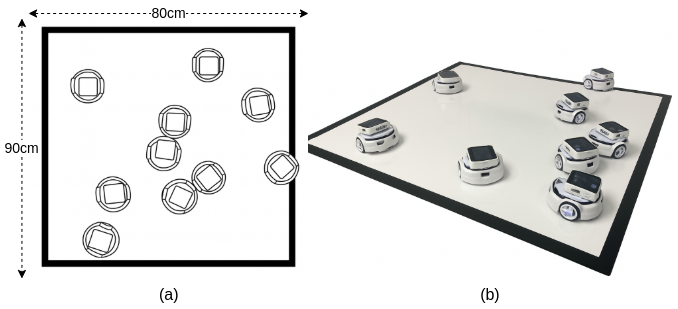
\includegraphics[width=0.49\textwidth]{arena.png}
    \caption{Experimental setup: (a) arena dimensions and (b) example of a Brownian locomotion experiment with 8 robots.}
    \label{fig:arena}
\end{figure}

%might have to explain contention and radio physical properties....

We explore three communication factors and their measurable effects (i) peer ordering, (ii) fixed per-robot message budgets, and (iii) per-packet stochastic transmission delays. We ask, \textbf{RQ1}: whether communication-aware peer ordering using \emph{link-quality} as a lightweight proxy for topology (see Section~\ref{sec:topology-inference}) changes network $QoS$, connection formation patterns, and time-to-consensus relative to stochastic ordering; \textbf{RQ2}: whether these factors influence information diffusion or convergence speed compared with one another; and \textbf{RQ3}: whether micro-delays between transmissions can mitigate collision bursts without harming delivery by measuring proxies such as latency and throughput.

\section{Related Work}
Island-model evolutionary algorithms in \cite{rucinski_impact_2010}, show that migration (genome exchange) topology and connectivity structure govern convergence dynamics not just the migration rate, with the Rastrigin function Eq. \ref{eq:rastrigin}, used to benchmark the performance of different asynchronous evolutionary algorithms. \\

In \cite{hauert_evolved_2009}, controllers are evolved for ad-hoc aerial relays without positional information, using periodic single-hop broadcasts to neighbours. This concept is leveraged on our experimental setting where the agents exploit link-quality proxies to bias their connections. In non-local communication schemes such as \cite{perrin_decentralised_2012}, network-wide epidemic broadcasting known as \emph{flooding} is used to accelerate the diffusion of information, for environmental mapping experiments. In contrast, our study uses \emph{unicast} peer-to-peer links at the data-link layer, enabling direct round-trip time measurements. \\

Constrained connectivity repeatedly appears beneficial. The \emph{"less is more"} effect in \cite{talamali_when_2021}, demonstrates that fewer links and lower swarm densities improve adaptation in swarm consensus tasks, by helping robots discard stale beliefs. A similar effect is also observed by \cite{hiraga_when_2023} over embodied evolution, where limiting the genome-exchange range can support the evolutionary search maintain higher diversity for longer and escape local optima. We explore similar properties which are discussed in Section-\ref{sec:discussion}, the main difference being the data-links used and our message prioritisation algorithm.  \\

Transmission timing also matters. Experiments from \cite{aust_hidden_2022} show that limiting the frequency of communication stabilises swarm behavior, while \cite{tsianos_impact_2012} explains that the speed of consensus among peers tolerates random transmission delays even when agents receive multiple out-of-order messages. Furthermore, non-radio data links have also been explored by \cite{trenkwalder_swarmcom_2020}, which shows that infra-red (IR) line-of-sight local communication can be used in swarms, some benefits include lower energy requirements per bit, moreover we note that IR has limits on bandwidth and bit error probability that scales with range. \\ 

Complementary work by \cite{rabbah_real_2021} examines real-time communication middleware for swarms at the application layer, addressing peer-to-peer IP protocols. In contrast we explore direct peer-to-peer exchange managed without any middleware. \\

% Over-the-air (OTA) mechanisms tailored to swarms have been explored by \cite{varadharajan_over--air_2018}, where updates are distributed as compact patches using gossip-style communication protocols to ensure version uniformity across large robot groups. We adapt this concept in Section-\ref{sec:ota} to support synchronised firmware across our deployment. \\


\section{Experimental Setting}

In this study, we use Eq. \ref{eq:rastrigin} to benchmark the evolutionary performance of the swarm. This global optimisation task was chosen to emulate evolutionary controller optimisation, while no controller was actually evolved the concept of robots sending and receiving genomes from their peers remains the same. \\

The environment for the experiments was a rectangular arena measuring 80x90cm without obstacles (Fig. \ref{fig:arena}a), where the initial positions, and number of the robots was determined by the experiment schedule (Table \ref{tab:exp_config}). Across the study, we evaluated swarm under different communication and system configurations. Each experiment manipulates a specific independent variable while holding all other conditions constant. These include:\\
% All of the experiments were conducted in the same room environment within the department of Engineering Mathematics at the University of Bristol.

\begin{itemize}
  \item \textbf{Swarm density}: The number of agents deployed simultaneously, ranging from 3 to 13.
  \item \textbf{Locomotion}: Robots were either \emph{stationary} or navigated using a \emph{Brownian motion} gait.
  \item \textbf{Topology inference}: Peer transmission priority was governed by either a \emph{stochastic} shuffle or a \emph{comm aware} ranking strategy based on link quality metrics.
  \item \textbf{Message limits}: A \emph{message budget} controlled how frequently agents could communicate with one another.
  \item \textbf{Transmission frequency}: Each transmission was optionally delayed by a random interval derived from the maximum observed peer latency.
\end{itemize}

Note that a detailed description of the communication independent variables is available in Section~\ref{sec:comm-layer}.

\subsection{Rastrigin Function}

The Rastrigin function is defined as follows:

\begin{equation}\label{eq:rastrigin}
f_R(\mathbf{x}) = 10n + \sum_{i=1}^{n} \left(x_i^2 - 10\cos(2\pi x_i)\right)
\end{equation}

Where $n$ is the number genes migrating between islands (robots). Whereas, $x$ is the individual genome being evaluated. The function has a global minimum at \( f_R(\mathbf{x}) = 0 \) \cite{rucinski_impact_2010}. Early single-robot trials showed that $n=10$ created enough search difficulty for performance to be measurable across swarm sizes.

\subsection{Robot Platform}\label{sec:robot_platform}
\begin{figure}[h]
    \centering
    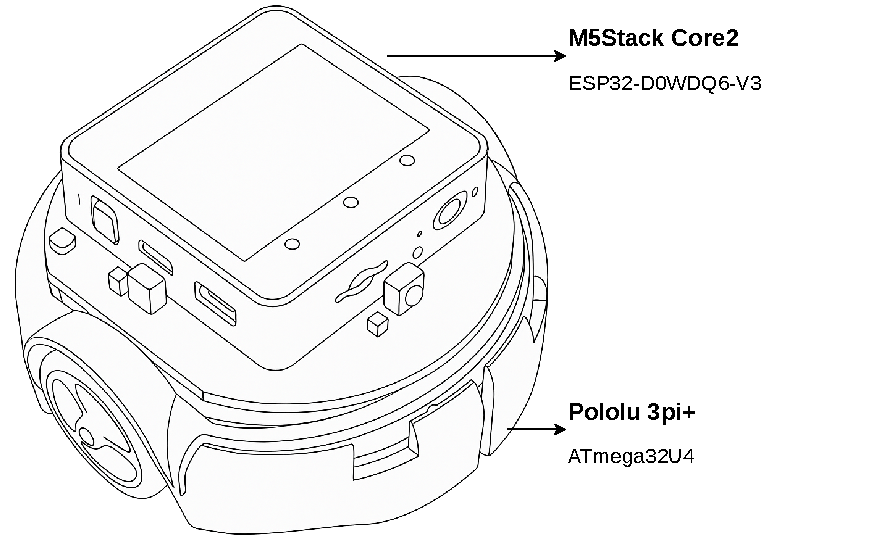
\includegraphics[width=0.45\textwidth]{B2.pdf}
    \caption{The Swarm-B2 platform: M5Stack Core2 and Pololu 3Pi+}
    \label{fig:B2}
\end{figure}

Table~\ref{tab:B2-hardware} summarizes the main hardware components of the Swarm-B2 platform used in this study [REF]. Devices coordinate via a $I^2C$ 100kHz bus. The ESP32 microcontroller runs dual-core FreeRTOS tasks, that logs real-time data to the local SD card, and manages communication using the ESP-NOW data link (2.4 GHz). \\

\begin{table}[h]
  \centering
  \caption{Swarm-B2 hardware stack}
  \label{tab:B2-hardware}
  \begin{tabular}{p{0.20\linewidth} p{0.18\linewidth} p{0.50\linewidth}}
    \toprule
    Component & Interface & Function \\
    \midrule
    M5Stack Core2 (240 MHz) & $I^2C$ Master       & Embedded evolution, ESP-NOW communication, data logging and user interface \\
    Pololu 3Pi+ (16 MHz)    & $I^2C$ Slave        & Locomotion using bumper and line following sensors \\
    \bottomrule
  \end{tabular}
\end{table}

The Pololu 3Pi+ is equipped with a line following sensor array and two bump sensors, which were used to navigate the around arena as the robots have no positional sensing. A \emph{Brownian-motion} gait was selected to maintain unbiased mobility across the arena and ensure constant movement. The gait code exposes the Pololu 3pi+ slave to the ESP32 master node, this interface lets the ESP32 act as a passenger with override, that can set speed scaling factors or raise \texttt{START}/\texttt{STOP} flags without touching the low-level control loop. Figure~\ref{fig:UI} shows the on-board display, used only for debugging and device status during development. A real-time clock (RTC) synchronised experiment runs across the swarm.

\section{Implementation}\label{sec:implementation}
Reliable and precise data logging is a pre-requisite for evaluating the communication performance and evolution dynamics of the swarm. To achieve this, our framework implements several mechanisms to capture and record key metrics which are explained in this section.

\subsection{System Architecture}\label{sec:architecture}

The firmware was implemented using the Espressif's ESP-IDF framework to provide real-time multitasking. Firmware updates and telemetry data capture are cloud enabled. Code that is written locally in VSCode (ESP-IDF v5.1.4) is rebuilt by GitHub Actions for validation. Only binaries that pass tests are signed and uploaded to an Amazon Web Services (AWS) S3 OTA bucket with a versioned register. On boot, each robot fetches the version register, streams any newer release into an idle OTA slot, and then resets with the latest firmware.

\begin{figure}[hb]
    \centering
    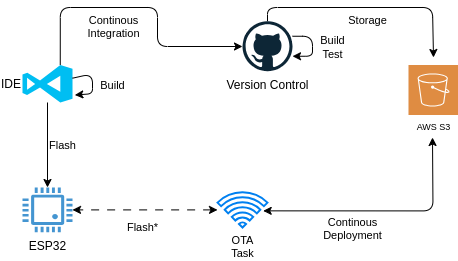
\includegraphics[width=0.45\textwidth]{architecture.png}
    \caption{Integrated architecture: Local development, GitHub repository, AWS S3 storage, and OTA updates.}
    \label{fig:cicd-architecture}
\end{figure}

Experiment schedules ran in batches. During execution, time-stamped messages and event logs are written to a local SD card. After execution, the robot uses WiFi to upload telemetry into an AWS S3 bucket. These files are serialised as JSON, tagged with the \texttt{experiment\_id}, and later processed with AWS Glue/Athena and visualised in PowerBI. This data processing pipeline, allowed us to harvest high-volumes of traceable log data per-robot and per-experiment (see Section~\ref{sec:evaluation-metrics}), while keeping the ESP-NOW data link isolated from Wi-Fi interference during experiments.

% \begin{figure}[H]
%     \centering
%     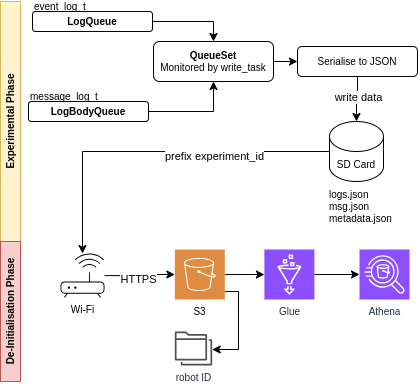
\includegraphics[width=0.45\textwidth]{data_store.png}
%     \caption{Internal data logging pipeline}
%     \label{fig:data-store}
% \end{figure}

\subsection{Embedded Evolution}\label{sec:embedded-evo}

The swarm uses a distributed genetic algorithm to find the global minimum for Eq. \ref{eq:rastrigin}. A visual representation of this is shown in Fig. \ref{fig:ga}. As the local population in each agent evolves, the swarm begins to communicate their local fitness and corresponding genome to their peers. \\

\begin{figure*}[t]
    \centering
    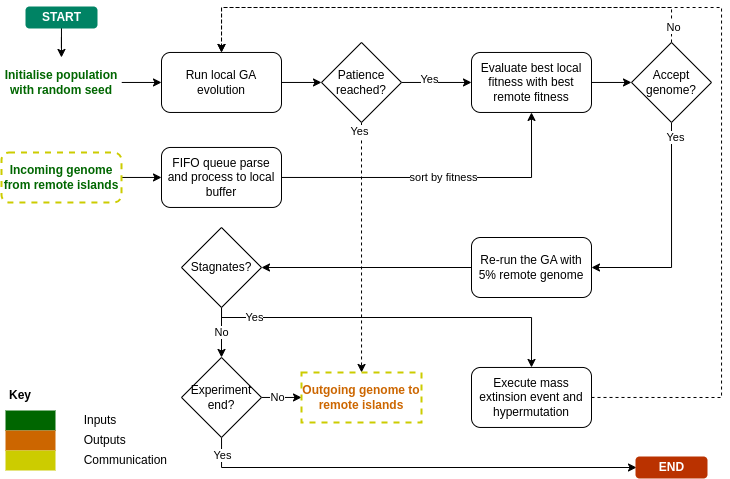
\includegraphics[width=1\textwidth]{ga.png}
    \caption{Distributed island-model GA executed on the ESP32 swarm}
    \label{fig:ga}
\end{figure*}

Our implementation employs an elitist migration strategy, this happens when the local GA reaches a patience threshold and the agent pushes its "best" (lowest fitness score) genome to other swarm members via ESP-NOW. The incoming remote genes from another peer are integrated into the local population by replacing the worst performing $5\%$ individuals, this value was chosen to preserve genomic high fitness locally. \\ 

To avoid stagnation over a local-minima and promote exploration across the swarm, a mass extinction event together with a hyper-mutation mechanism tracks consecutive non-improving generations \cite{krink_self-organized_2001}. In each agent, if the local population's fitness remains stale for over 3 seconds, the mutation probability is temporarily increased and the lowest performing half of the population is re-initialised. \\ 

Evolution continues locally until the experiment ends, triggered either by (i) discovering the global optimum (fitness = 0) or (ii) a 60 s timeout with no convergence. Two FreeRTOS tasks run in parallel, one executes the GA and the other handles ESP-NOW messaging. During shutdown, the \texttt{espnow\_task} flushes any queued packets. Then evolutionary and communication files are uploaded to the telemetry S3 over HTTPS.

\subsection{Message Structure}

We evaluate robot-to-robot communication with a fixed ESP-NOW message schema (Table \ref{tab:out_message}), floats are rounded to $3d.p.$ to send the message in a single transmission. Implications of this design choice are discussed in Section~\ref{sec:discussion}.

\begin{table}[H]
  \centering
  \caption{Message structure used for ESP-NOW fitness value and genome exchange}
  \label{tab:out_message}
  \begin{tabular}{l l p{4cm}}
    \toprule
    \textbf{Field} & \textbf{Type} & \textbf{Description} \\
    \midrule
    \texttt{log\_id} & uint32\_t & Unique internal identifier of the event.\\
    \texttt{robot\_id[5]} & char & MAC identifier for the sender robot plus a null terminator.\\
    \texttt{log\_datetime} & time\_t & Timestamp based on the internal RTC.\\
    \texttt{message[128]} & char & Content of the message including the fitness value and the 10-gene genome delimited by "$|$".\\
    \bottomrule
  \end{tabular}
\end{table}

\subsection{Communication Layer}\label{sec:comm-layer}

In contrast to previous work by \cite{rabbah_real_2021} that explored decentrilised IP communication protocols using middleware in swarms, we exploit the ESP32s Medium Access Control (MAC) layer to keep  packet timing and load directly measurable.To do this, we had to implement ESP-NOW by pre-registering the MAC addresses of all peers in each agent's firmware, enabling direct unicast communication between robots. We do not view this as a hard scalability limit in the swarm paradigm, as \cite{varadharajan_over--air_2018} explains that gossip-style OTA propagation can disseminate firmware across the swarm, allowing MAC registers to scale without central coordination. \\

Our design uses push only event-driven peer-to-peer messaging, where each device transmits data to peers (migration) without waiting for requests. Using this scheme avoids the complexity of pull-based communication protocols. Recall from Section~\ref{sec:embedded-evo} that only local elite genomes migrate, this takes place asynchronously between islands as each robot's GA reaches migration thresholds at different times. Because of this, incoming messages are handled by a first-in/first-out queue and buffered locally for later processing. This allowed internal task operations to continue uninterrupted, at the cost of internal memory, from pilot experiment we set the queue size to 40 (~8KB). \\

Social evidence, in our case is present in the form of the communication quality that arises from migration. Specifically from the latency and Received Signal Strength Indicator (RSSI) that a peer perceives relative to other peers. We use this social evidence to inform our communication strategy and adapt the following policies. \\

\subsubsection{Topology Inference}\label{sec:topology-inference}

We investigate the impact of two communication schemes, based on the social evidence retained locally per-peer. These schemes were designed to influence the priority and order with which each agent sends messages. We use the social evidence as a proxy to infer the topology, under the assumption that distant islands would exhibit different link quality characteristics. These are implemented as follows:

\begin{itemize}
    \item \emph{Stochastic}: Each agent calls a random seed to apply a Fisher-Yates shuffle \cite{fisher_statistical_1963} over the list of peer MAC addresses, sorting them before sending messages to \emph{all peers}. No social evidence bias is used, every order permutation is equally likely.
    \item \emph{Comm aware}: Each agent ranks its peers based on the most recent measurements of latency and RSSI. Peers with unknown metrics (at initialisation) are prioritised first to ensure social evidence is available. Then, peers are scored by normalizing both latency and RSSI, and those only in the \emph{worst half} (highest latency, lowest RSSI) are messaged.
\end{itemize}

For \emph{stochaistic}, the shuffle is defined in Eq.~\ref{eq:fy-shuffle}, where ($j_i$) is a random index drawn from a uniform distribution. $\sigma$ is the random permutation of MAC addresses for each $i$ peer. We can think of this scheme as a \emph{pseuso-broadcast} using unicast communication, as the genome is sent to all peers with negligible delays between transmissions.

\begin{equation}\label{eq:fy-shuffle}
\sigma \;=\; \prod_{i=n}^{2} \bigl(i,\, j_i\bigr), 
\qquad j_i \sim \mathrm{Uniform}\{1,\dots,i\}
\end{equation}

Whereas for \emph{comm aware}, the scoring for peer $i$ ranking is defined in Eq.~\ref{eq:comm-aware}. Here, the round-trip latency $l$ can be measured via acknowledgements (ACKS). The RSSI $r$ is reported by the ESP-NOW send callback after each successful transmission. If multiple messages have been sent, only the most recent metrics stay in memory. Note that both RSSI and latency are scored equally.

\begin{equation}\label{eq:comm-aware}
Score_i =
\frac{l_i - l_{\min}}{l_{\max} - l_{\min}} +
\frac{r_{\max} - r_i}{r_{\max} - r_{\min}}
\end{equation}

\subsubsection{Message Budgets}\label{sec:limited-rate}

Inspired by the reported “less-is-more” effects, we cap the number of migration messages that each robot may broadcast (Eq.~\ref{eq:msg_budget}). Each agent is given a message budget $B$ per sliding time window $W$. Once the budget is exhausted, the robot stays silent until the window advances, no matter how often its onboard genetic algorithm requests migration.  Different from earlier IR-based systems that relied on a short-range \emph{narrowcast} channel \cite{aust_hidden_2022}, we deliver the message to all peers using the topology inference schemes discussed previously.

\begin{equation}\label{eq:msg_budget}
\forall t:\quad M_W(t)=\sum_{i}\mathbf{1}_{\{t-W< t_i \le t\}} \le B
\end{equation}

Here, $t_i$ are the send times, $M_W(t)$ is the number of broadcast messages sent in the last $W=8$s, and the budget is fixed at $B=1$. These values were chosen after pilot tests showed that, without the budget, each peer emitted roughly 15 messages per experiment, effectively limiting migration by half. \\

\subsubsection{Transmission Frequency}\label{sec:transmission-frequency}

To further explore the communication behaviour of the swarm under simultaneous transmission conditions, we modulate the migration interval between islands. Each migration is postponed by random delay drawn from the highest peer-to-peer latency observed so far, which is estimated from the latest ACK round-trip times on every link, described by Eq.~\ref{alg:transmission_freq}:

\begin{equation}\label{alg:transmission_freq}
\Delta t \sim \mathrm{Uniform}\bigl(0,\,L_{\max}\bigr), 
\qquad
L_{\max} = \max_{j}\{\tau_{j}\}
\end{equation}

where ($\tau_{j}$) is the one-hop latency to peer ($j$). If random mode is disabled, ($\Delta t = 0$) and messages are sent immediately by calling \texttt{esp\_now\_send}. The intention of this approach is to control the transmission of messages in a stochastic manner to reduce unintended channel contention in the swarm network.

\subsection{Communication Performance Metrics}\label{sec:evaluation-metrics}

To evaluate the quality of the communication in the swarm, each robot records granular \emph{sender-receiver}: latency $l$ (ms), RSSI $r$ (dBm), net kilobyte rate $t$ (Kbps), transmission-error flags $e$, and per-core CPU load $u$. These raw logs are post-processed by the data pipeline previously detailed in Section \ref{sec:architecture}. AWS then computes the aggregated per-device and per-experiment metrics, (i) $L$ \emph{mean latency}, the time taken for a message to be sent and acknowledged, (ii) $J$ \emph{mean jitter (ms)}, the standard deviation of successive latencies, (iii) $E$ \emph{mean error rate (\%)}, the percentage of messages that were sent but not acknowledged, and (iv) $T$ \emph{mean throughput (kbps)}, the data is successfully transferred by each agent. To assess overall network performance, a QoS score was computed as:

\begin{equation}
\mathrm{QoS} = w_0 \cdot (1 - \hat{L}) + w_1 \cdot (1 - \hat{J}) + w_2 \cdot (1 - \hat{P}) + w_3 \cdot \hat{T}
\end{equation}

Where, $\hat{L}$, $\hat{J}$, $\hat{E}$, $\hat{T}$ are the normalised global metrics aggregated at the experiment-level in the range of $[0,1]$ and the weights $w_i$ are defined in Table \ref{tab:qos}. A higher QoS value indicates better overall network communication performance.

\begin{table}[H]
\centering
\caption{QoS utility function weights for different swarm robotics applications}
\label{tab:qos}
  \begin{tabular}{@{} lcccc p{3.5cm} @{}}
  \toprule
  \textbf{QoS} & \textbf{$w_0$} & \textbf{$w_1$} & \textbf{$w_2$} & \textbf{$w_3$} & \textbf{Application} \\
  \midrule
  $QoS_c$      & 0.5  & 0.25   & 0.15   & 0.1     & Swarm consensus and voting     \\
  $QoS_s$      & 0.15 & 0.15   & 0.50   & 0.2     & Swarm sparse deployments       \\
  \bottomrule
  \end{tabular}
\end{table}

\section{Results}\label{sec:results}

As shown in Figure \ref{fig:topology}(a), the latency and jitter of the swarm network differ significantly between topology inference schemes. Across experiments the \emph{COMM AWARE} topology strategy generally achieves lower latency and more stable delivery compared to the \emph{STOCHASTIC} mode. Figures \ref{fig:topology}(b) and \ref{fig:topology}(c) show that throughput is highest in unconstrained conditions, and drops with the introduction of message budgets. \emph{STOCHASTIC} communication yields higher raw throughput but also has a wider range of variability.

\begin{figure*}[h]
    \centering
    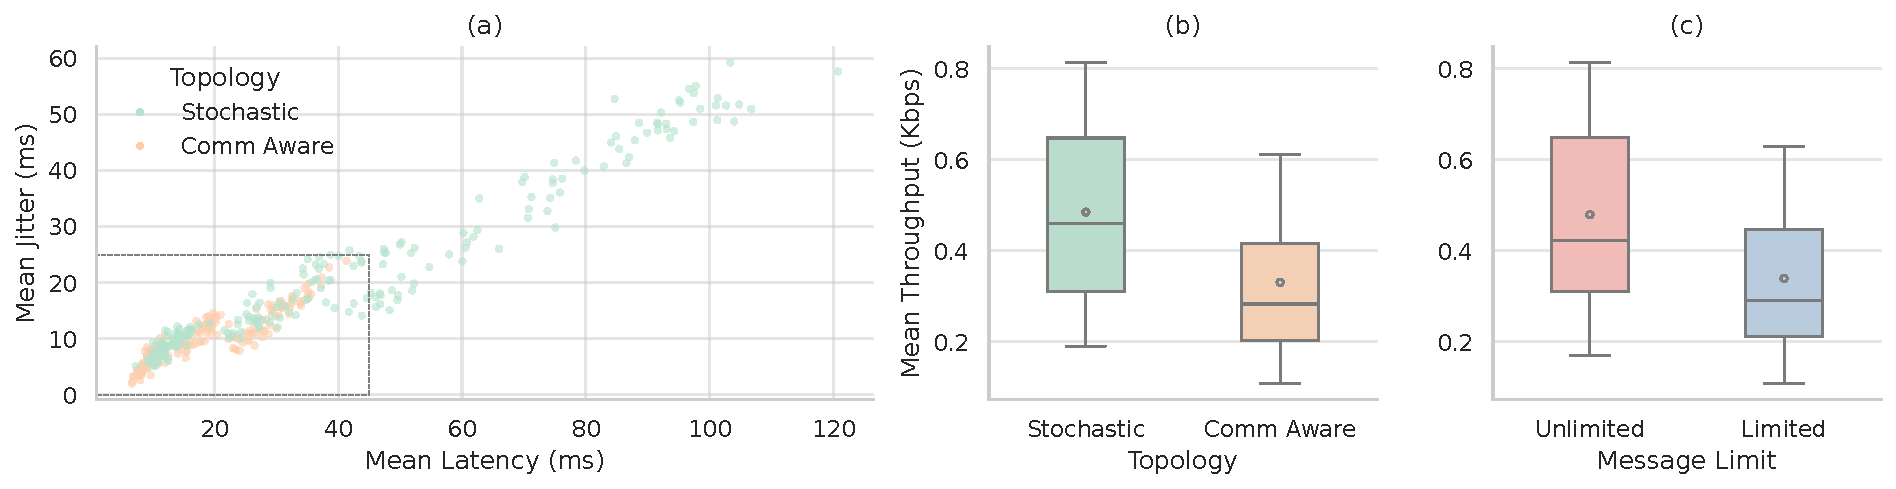
\includegraphics[width=1\textwidth]{topology_impact.pdf}
    \caption{(a) Latency and Jitter relationship under varying topology schemes, (b)(c) throughput distribution under topology and message limit variables}
    \label{fig:topology}
\end{figure*}

Figure \ref{fig:performance}(a) shows that larger swarms converge to lower mean fitness scores, indicating improved global convergence as agent density increases. Figure \ref{fig:performance}(b) presents the adaptation rate over time. Swarms using the \emph{STOCHASTIC} communication scheme tend to converge more rapidly, with approximately $80\%$ of the agents reaching the best-known solution roughly 20 seconds earlier than those using the \emph{COMM AWARE} strategy. Here, adaptation rate is defined as the proportion of agents that share the current lowest fitness score, averaged over 2-second windows.

\begin{figure*}[h]
    \centering
    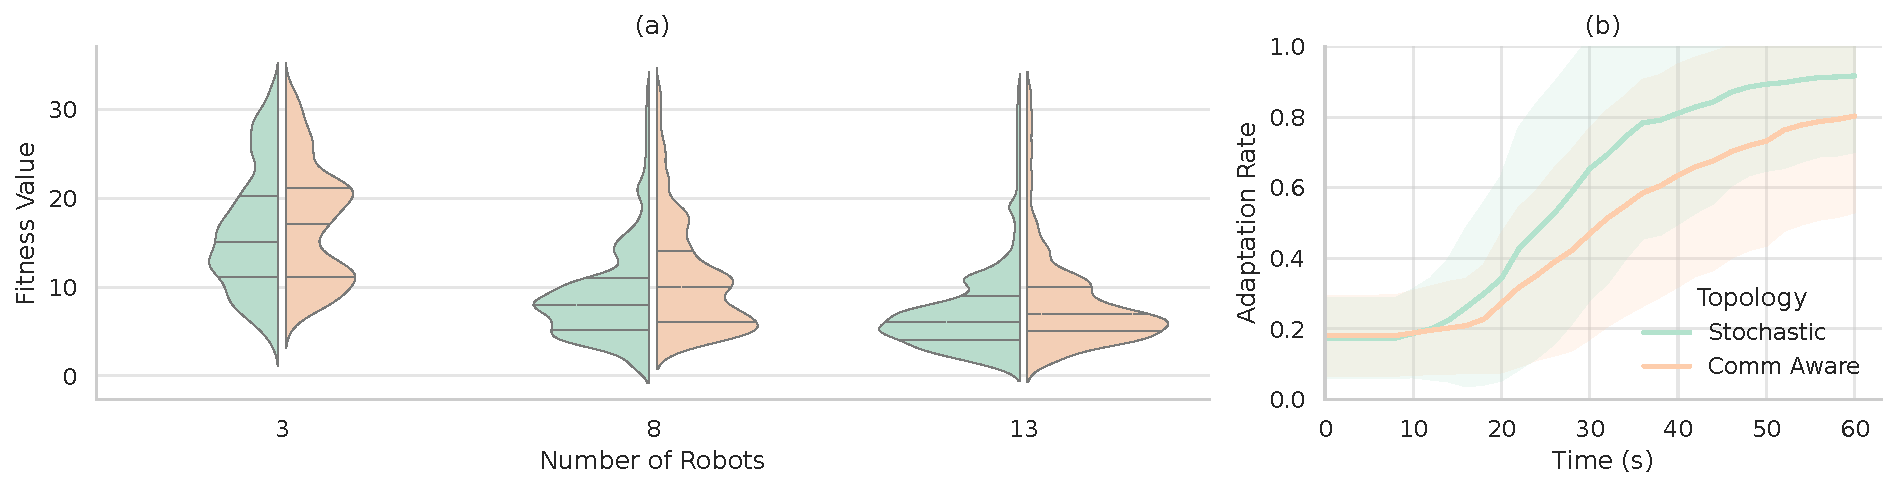
\includegraphics[width=1\textwidth]{performance_impact.pdf}
    \caption{(a) Mean device fitness values across different swarm sizes, (b) mean cumulative percentage of agents converging to the lowest fitness value across $2s$ windows}
    \label{fig:performance}
\end{figure*}

Figure \ref{fig:error-rates}(a) shows the mean packet error rate across different swarm densities. The error rates remain low overall but increase with the swarm size, and it is particularly impacted by the \emph{STOCHASTIC} scheme (Figure \ref{fig:error-rates}(b)).

\begin{figure}[H]
    \centering
    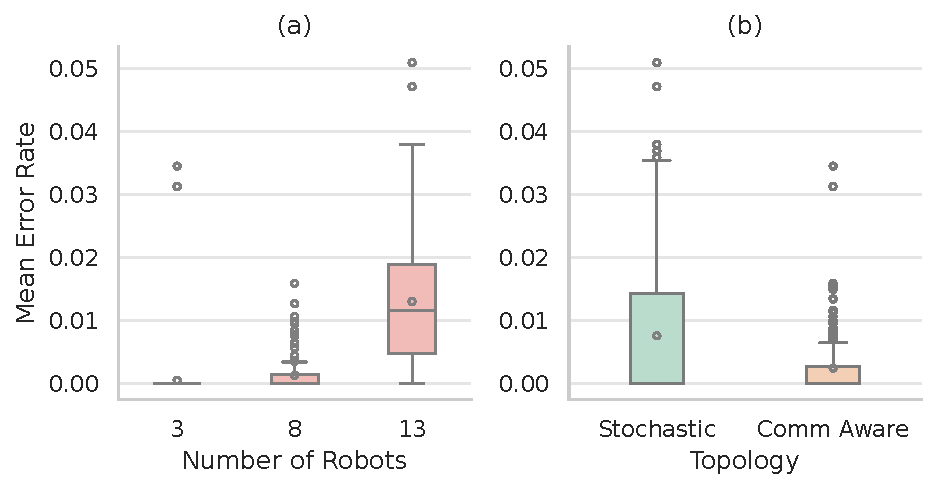
\includegraphics[width=0.47\textwidth]{reliability_impact.pdf}
    \caption{(a) Mean error rates by device across varying swarm sizes, (b) mean error rate for different topology inference schemes}
    \label{fig:error-rates}
\end{figure}

With regards to locomotion Figure \ref{fig:rssi}(a) shows that Brownian motion results in slightly improved RSSI values, indicating more stable connections compared to static swarms. Whereas \ref{fig:rssi}(b) suggests no statistical difference between RSSI values across topology inference schemes.

\begin{figure}[H]
    \centering
    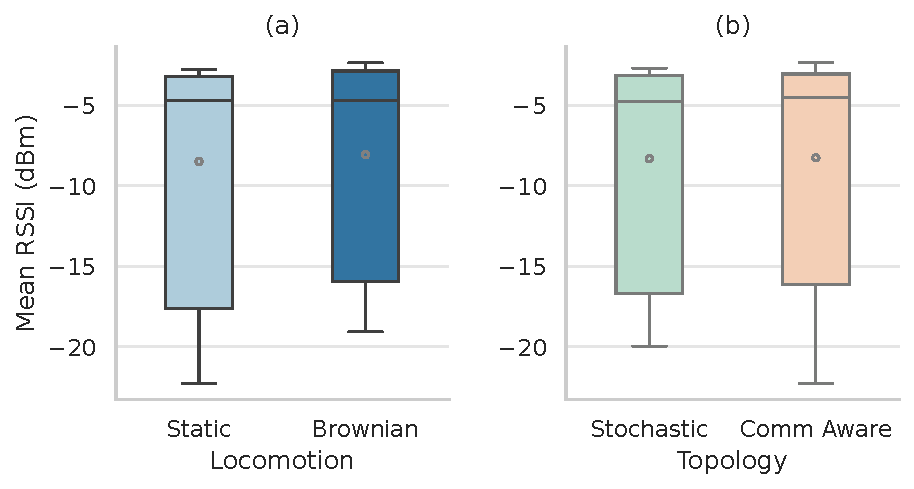
\includegraphics[width=0.47\textwidth]{speed_impact.pdf}
    \caption{(a) Mean RSSI values across different locomotion modes, (b) mean RSSI values accross different topology inference schemes}
    \label{fig:rssi}
\end{figure}

Considering the impact of transmission frequency for experiments under the STOCHASTIC scheme, Figure \ref{fig:frequency}(a) shows that modulated transmission policies also restrict the network to lower latency and jitter though not to the same degree. Figure \ref{fig:frequency}(b) illustrates how latency varies over time under different transmission settings, with modulated policies achieving lower more stable latencies. Figure \ref{fig:frequency}(c) shows that throughput is generally similar between policies, a contrast compared to the topology inference schemes. Similar to performance under varying topology inference conditions, the performance for alternating transmission policies remains impacted mainly by the increase in swarm density Figure \ref{fig:f-performance}(a). Moreover, the adaptation rate between transmission policies remains similar Figure \ref{fig:f-performance}.\\

\begin{figure*}[h]
    \centering
    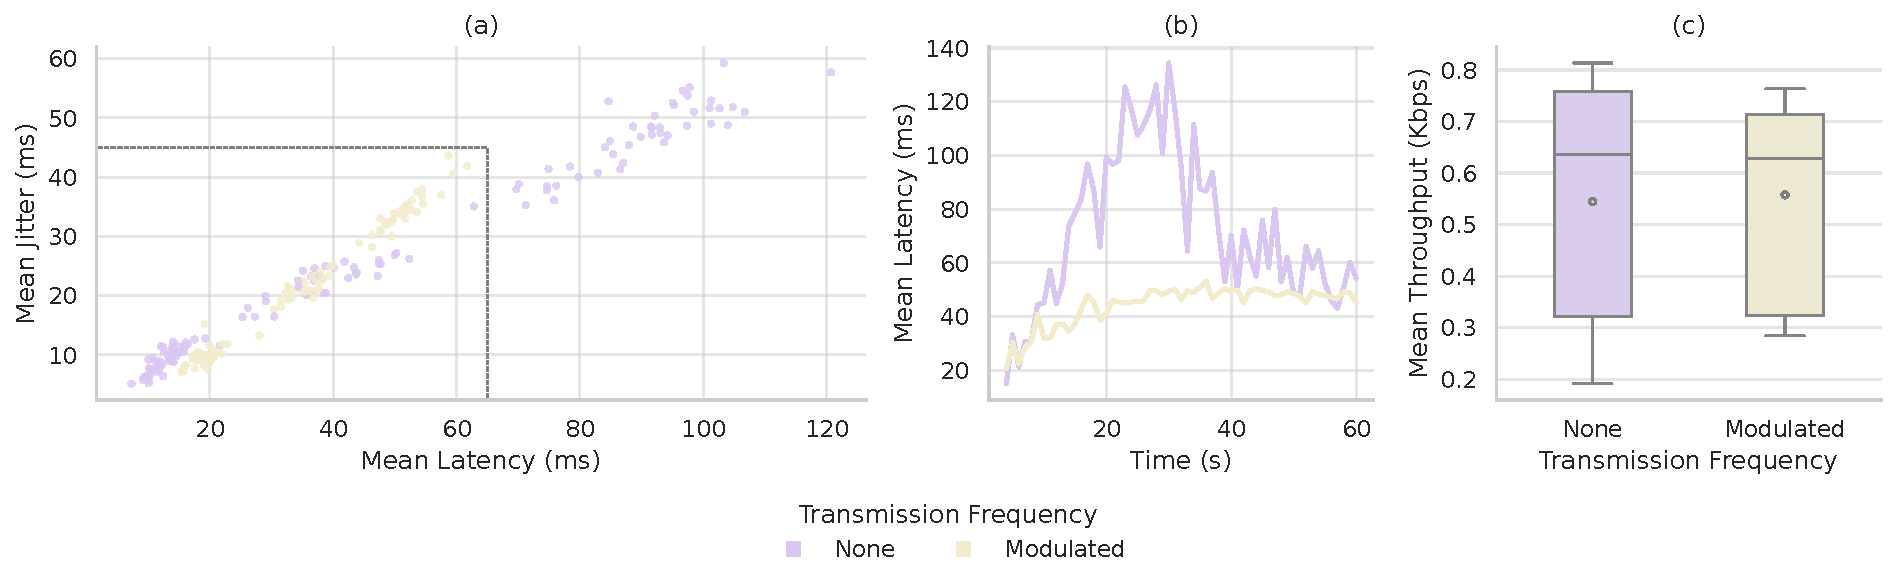
\includegraphics[width=1\textwidth]{frequency_impact.pdf}
    \caption{(a) Latency and Jitter relationship under varying transmission policies, (b) latency across time by transmission setting, (c) throughput distribution by transmission setting}
    \label{fig:frequency}
\end{figure*}

\begin{figure*}[h]
    \centering
    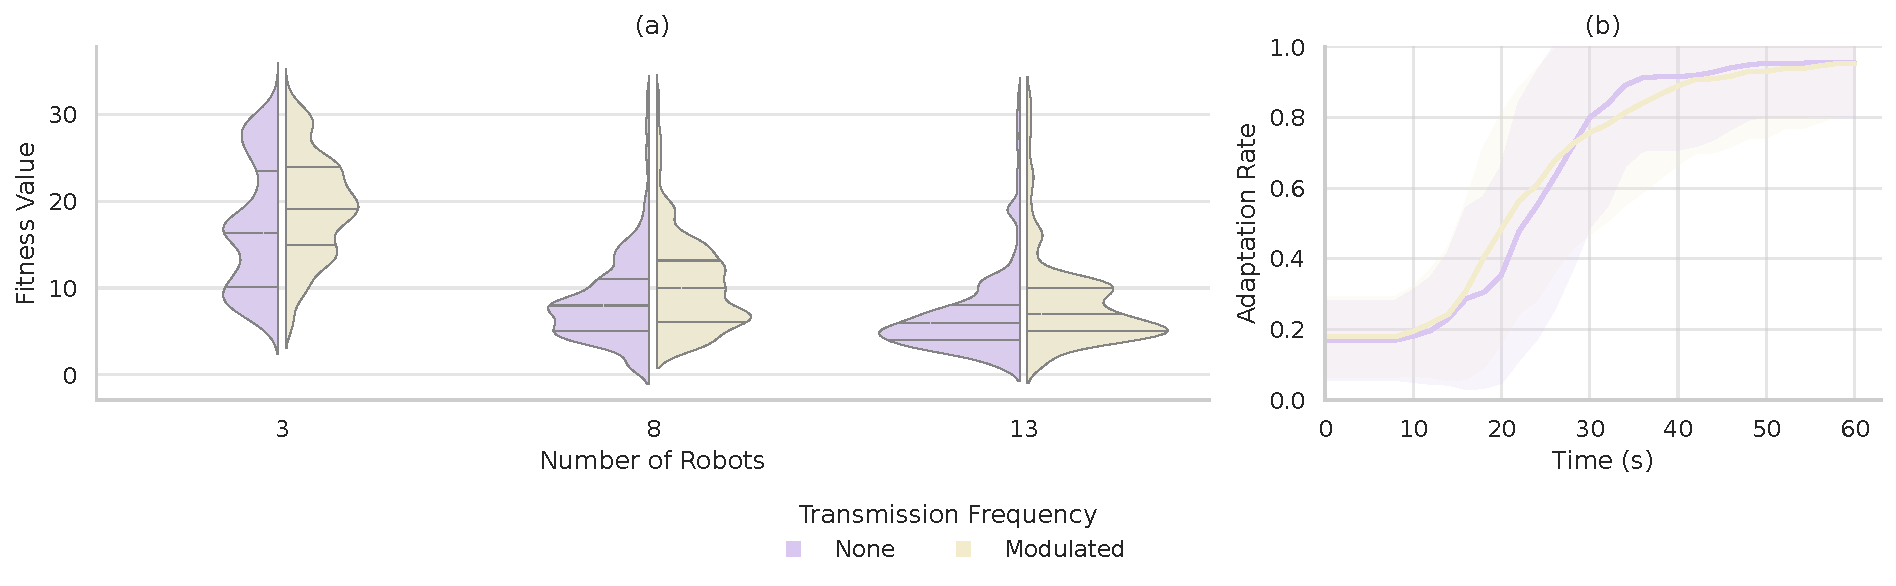
\includegraphics[width=1\textwidth]{f_performance_impact.pdf}
    \caption{(a) Mean device fitness values across different swarm sizes, (b) mean cumulative percentage of agents converging to the lowest fitness value across $2s$ windows}
    \label{fig:f-performance}
\end{figure*}

An evaluation of the characteristics of the QoS metrics for the 13-agent swarm is shown in Figure \ref{fig:qos}. Key observations include, (i) COMM AWARE topology inference achieves high QoS metrics, (ii) modulated transmission also scores high in QoS but tends to score higher in $QoS_s$, (iii) message limits do not have a clear effect on QoS, both kernel densities overlap each other.

\begin{figure*}[h]
    \centering
    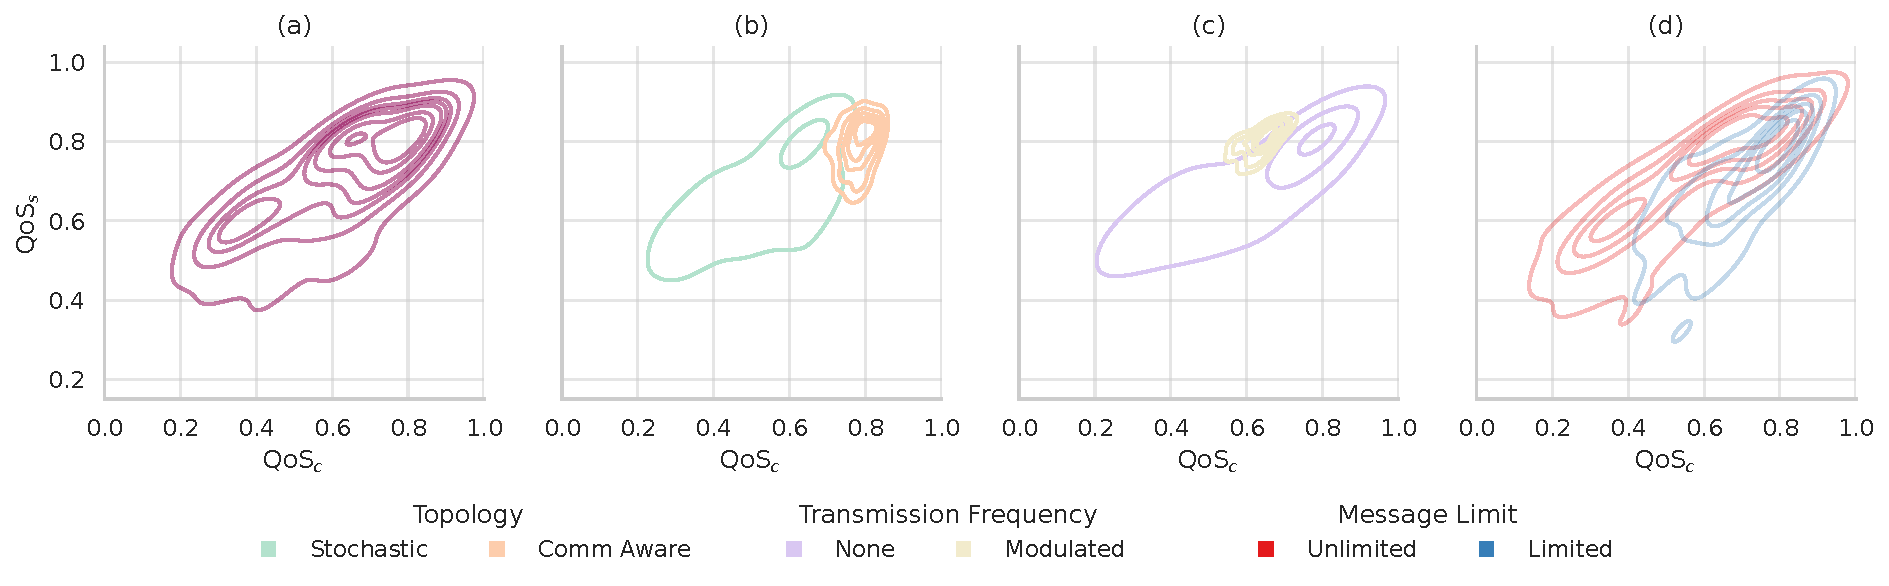
\includegraphics[width=1\textwidth]{qos_impact.pdf}
    \caption{Kernel-density contours showing the joint distribution of two QoS metrics (x: $QoS_c$, y: $QoS_s$) for a 13-agent swarm. (a) pooled across all experimental factors, (b) split by communication topology, (c) split by transmission frequency policy, (d) split by message limit setting}
    \label{fig:qos}
\end{figure*}

\renewcommand{\arraystretch}{0.9}  
\begin{table*}[ht]
\scriptsize
\centering
\caption{Experimental configurations}
\label{tab:exp_config}
\begin{tabular}{c|c|c|c|c|c|c|c|c|c|c}
\toprule
\textbf{Robots} & \textbf{Topology} & \textbf{Locomotion} & \textbf{Message Limit} & \textbf{Transmission} & \textbf{Latency (ms)} & \textbf{Jitter (ms)} & \textbf{Error Rate (\%)} & \textbf{Throughput} & \textbf{QoS\_c} & \textbf{QoS\_s} \\
\midrule
2 (Baseline) & Stochastic & Static & Unlimited & None & -- & -- & -- & -- & -- & -- \\
\midrule
\multirow{10}{*}{3}
  & \multirow{5}{*}{Stochastic}
    & \multirow{2}{*}{Static}
                 & Unlimited & None      & -- & -- & -- & -- & -- & -- \\
  &   &          & Unlimited & Modulated & -- & -- & -- & -- & -- & -- \\
  &   &          & Limited   & None      & -- & -- & -- & -- & -- & -- \\
  \cmidrule{3-11}
  &   & \multirow{2}{*}{Brownian}
                 & Unlimited & None      & -- & -- & -- & -- & -- & -- \\
  &   &          & Unlimited & Modulated & -- & -- & -- & -- & -- & -- \\
  &   &          & Limited   & None      & -- & -- & -- & -- & -- & -- \\
  \cmidrule{2-11}
  & \multirow{5}{*}{Comm Aware}
    & \multirow{2}{*}{Static}
                 & Unlimited & None      & -- & -- & -- & -- & -- & -- \\
  &   &          & Limited   & None      & -- & -- & -- & -- & -- & -- \\
  \cmidrule{3-11}
  &   & \multirow{2}{*}{Brownian}
                 & Unlimited & None      & -- & -- & -- & -- & -- & -- \\
  &   &          & Limited   & None      & -- & -- & -- & -- & -- & -- \\
\midrule
\multirow{10}{*}{8}
  & \multirow{5}{*}{Stochastic}
    & \multirow{2}{*}{Static}
                 & Unlimited & None      & -- & -- & -- & -- & -- & -- \\
  &   &          & Unlimited & Modulated & -- & -- & -- & -- & -- & -- \\
  &   &          & Limited   & None      & -- & -- & -- & -- & -- & -- \\
  \cmidrule{3-11}
  &   & \multirow{2}{*}{Brownian}
                 & Unlimited & None      & -- & -- & -- & -- & -- & -- \\
  &   &          & Unlimited & Modulated & -- & -- & -- & -- & -- & -- \\
  &   &          & Limited   & None      & -- & -- & -- & -- & -- & -- \\
  \cmidrule{2-11}
  & \multirow{5}{*}{Comm Aware}
    & \multirow{2}{*}{Static}
                 & Unlimited & None      & -- & -- & -- & -- & -- & -- \\
  &   &          & Limited   & None      & -- & -- & -- & -- & -- & -- \\
  \cmidrule{3-11}
  &   & \multirow{2}{*}{Brownian}
                 & Unlimited & None      & -- & -- & -- & -- & -- & -- \\
  &   &          & Limited   & None      & -- & -- & -- & -- & -- & -- \\
\midrule
\multirow{10}{*}{13}
  & \multirow{5}{*}{Stochastic}
    & \multirow{2}{*}{Static}
                 & Unlimited & None      & -- & -- & -- & -- & -- & -- \\
  &   &          & Unlimited & Modulated & -- & -- & -- & -- & -- & -- \\
  &   &          & Limited   & None      & -- & -- & -- & -- & -- & -- \\
  \cmidrule{3-11}
  &   & \multirow{2}{*}{Brownian}
                 & Unlimited & None      & -- & -- & -- & -- & -- & -- \\
  &   &          & Unlimited & Modulated & -- & -- & -- & -- & -- & -- \\
  &   &          & Limited   & None      & -- & -- & -- & -- & -- & -- \\
  \cmidrule{2-11}
  & \multirow{5}{*}{Comm Aware}
    & \multirow{2}{*}{Static}
                 & Unlimited & None      & -- & -- & -- & -- & -- & -- \\
  &   &          & Limited   & None      & -- & -- & -- & -- & -- & -- \\
  \cmidrule{3-11}
  &   & \multirow{2}{*}{Brownian}
                 & Unlimited & None      & -- & -- & -- & -- & -- & -- \\
  &   &          & Limited   & None      & -- & -- & -- & -- & -- & -- \\
\bottomrule
\end{tabular}
\end{table*}


\section{Discussion}\label{sec:discussion}
%need to rewrite this and remove flooding.
Results for our hypotheses are as follows. \textbf{H1} is supported: \emph{COMM AWARE} achieves lower median latency ($\delta$ XX ms) and tighter jitter than \emph{STOCHASTIC}. \textbf{H2} is partially supported: message budgets slow diffusion and curb collisions yet do not prevent convergence, however the effect size is modest compared with topology choice. \textbf{H3} is supported: a delay capped by recent peer latency reduces contention, stabilises latency (jitter $YY\%$), and maintains throughput relative to pure flooding.\\

Across conditions, reductions in end-to-end latency are explained mainly by the number of links the swarm forms rather than by capping the number of transmissions, achieving below $50ms$ comparable to simulation conditions in \cite{hauert_evolved_2009}. Under \emph{STOCHASTIC} scheduling the pseudo-broadcasting behaviour of the swarm rapidly increases unique connections, which raises contention. In \emph{COMM AWARE}, reduced link formation avoids bursts of transmission, producing lower median latency and jitter at the cost of throughput. The time-snapshots of inferred topologies in Fig. \ref{fig:convergence} illustrate this mechanism directly, with \emph{STOCHASTIC} creating denser transient link sets than \emph{COMM AWARE} over comparable intervals. In this elitist island-model, slower mixing between islands can be useful. Limiting link formation in \emph{COMM AWARE} reduces premature convergence, allowing for a more diverse genome to persist and be explored longer. This aligns with the observation that overall fitness improves primarily with agent count (Fig. \ref{fig:performance}a), while the fastest adaptation rates arise under the \emph{STOCHASTIC} scheme where information diffuses quickly (Fig. \ref{fig:f-performance}b).\\

\begin{figure*}[h]
    \centering
    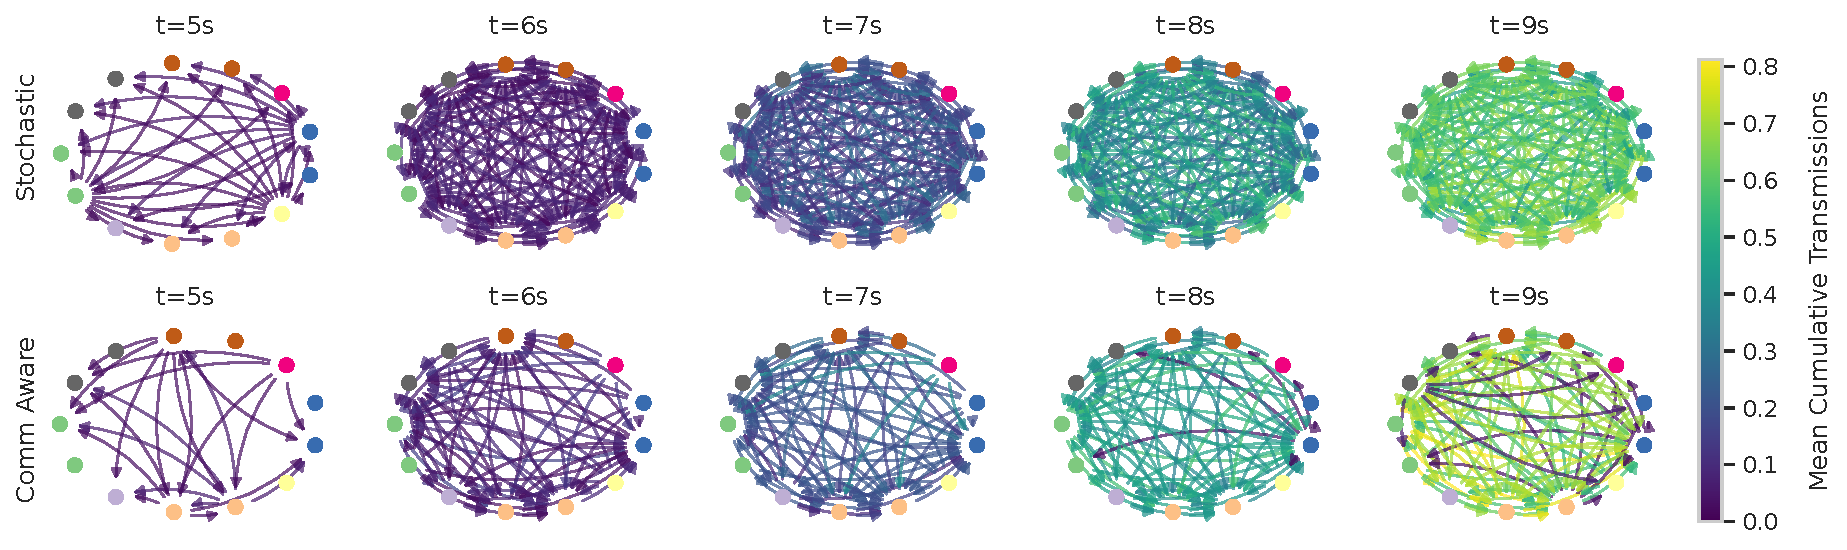
\includegraphics[width=1\textwidth]{convergence_impact.pdf}
    \caption{Temporal snapshots of inferred communication topologies for a 13-agent swarm. Rows: inference scheme, columns: time samples. Nodes are on a fixed circular layout, edges show inferred links and its colour indicates mean cumulative transmissions per node.}
    \label{fig:convergence}
\end{figure*}

\emph{COMM AWARE} attains consistently high $QoS$ values by suppressing jitter and keeping low latencies, while \emph{STOCHASTIC} achieves higher raw throughput but with wider variability and higher error rates as agent density grows. Kernel-density plots of $QoS_c$ against $QoS_cs$ in Fig. \ref{fig:qos} show \emph{COMM AWARE} achieving an overall improved service relative to the overall distribution, whereas frequency modulated \emph{STOCHASTIC} shifts mass toward $QoS_s$, reflecting higher throughputs with smoother latency over time.
Error rate increases with swarm size (Fig. \ref{fig:error-rates}), independent of locomotion, and becomes most pronounced under \emph{STOCHASTIC} at 13 robots—consistent with more concurrent transmissions and higher collision probability as unique links accumulate over time (Fig. \ref{fig:unique-connections}). This could explain why differences between policies are less pronounced at lower densities (3 to 8 robots) and widen at 13.\\

\begin{figure}[H]
    \centering
    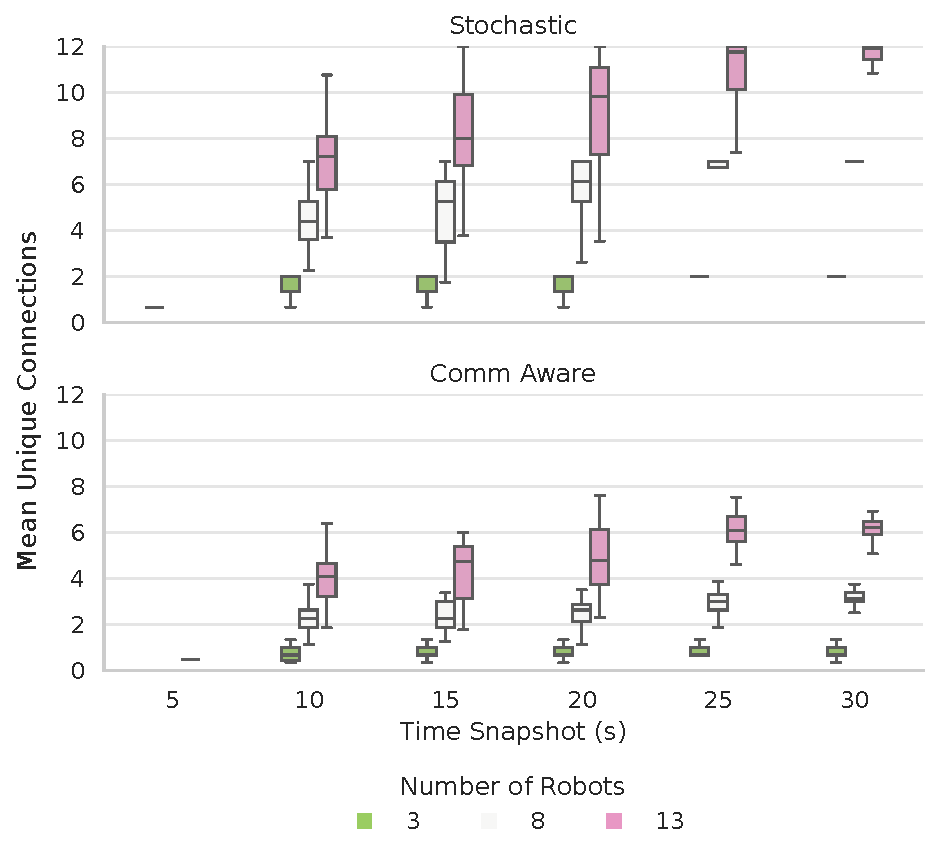
\includegraphics[width=0.46\textwidth]{unique_connections.pdf}
    \caption{Per-peer number of mean connections formed by time snapshot up to 30 seconds for both topology inference schemes}
    \label{fig:unique-connections}
\end{figure}

Results shown in Fig. \ref{fig:rssi}, indicate that RSSI does not meaningfully distinguish topology schemes in the arena used for the experiments, which means that the \emph{COMM AWARE} scheme is effectively ranking by latency. Brownian motion yields a slight RSSI improvement relative to static trials, plausibly by incidental repositioning into stronger links though verifying this would require sparser layouts or larger arenas.

Introducing frequency modulation under the \emph{STOCHASTIC} scheme smooths latency trajectories (Fig. \ref{fig:frequency}(b)) without sacrificing throughput, and preserves fast adaptation relative to \emph{COMM AWARE}. Validating the findings of \cite{tsianos_impact_2012}, the swarm can tolerate transmission delays and attain similar fitness relation compared to have no modulation. For tasks where rapid environment updates matter such as in \cite{perrin_decentralised_2012}, this policy provides a low complexity alternative to flooding, supported with a gentler latency profile.

Using the fixed ~145-byte genome structure (\texttt{OUT\_MESSAGE\_T}) in a single channel operation, we observe that GA performance is not capped by the aggregate throughput of the swarm. Having said that, we cannot ruleout the impact of a varying payload structure and single channel with respect to the GA without further experiments (e.g. partial genomes transfer, non-elitist migrants). Aditionally, more data would be needed to test whether the results gathered in this study remains the same as the messages grow closer to or beyond ESP-NOW 250-byte payload. We suspect that increasing the message size beyond the payload limits will introduce introduce challenges in asynchronous message processing as the local buffer would need to grow to prevent information loss and the subsequent compute requirements will increase as well.\\

Energy consumption matters. Broadcast-heavy policies increased CPU utilisation (Fig. \ref{fig:cpu-util}) and correlated with faster battery depletion during testing, whereas policies that constrain link formation (\emph{COMM AWARE}) reduced contention and processing load, extending runtime. For context, ESP-NOW transmit currents on ESP32 are typically an order of magnitude higher than BLE ($\approx100mA$ vs $\approx15mA$ during TX), so depending on the application, swarms may need to prioritise message budgets and partial link formation over peak performance. This trade-off is not abstract, in the author's current role at Unilode Aviation Solutions the operator of the largest globally distributed aviation IoT gateway network—battery longevity outranks other $QoS$ metrics because asset maintenance for sparsely distributed assets (agents) is measured in years rather than days.\\

\begin{figure}[H]
    \centering
    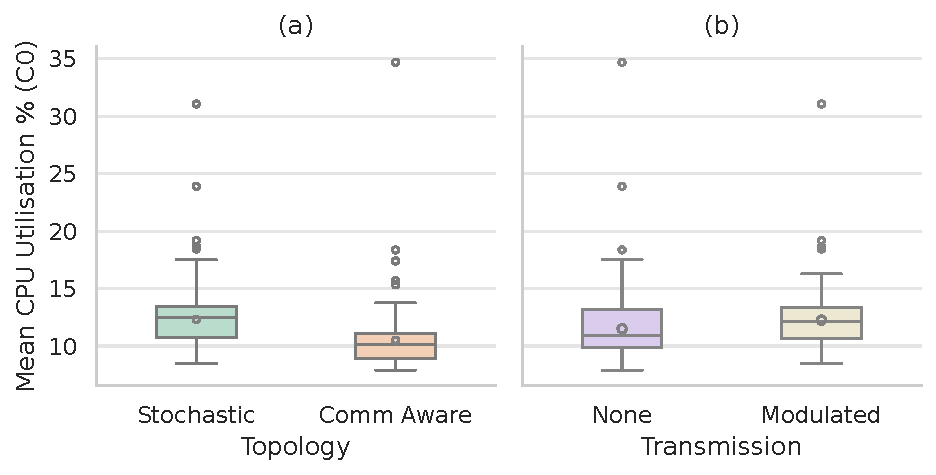
\includegraphics[width=0.46\textwidth]{cpu_util.pdf}
    \caption{Core 0 utilisation by communication policy, excluding message limited experiments}
    \label{fig:cpu_util}
\end{figure}

\subsection{Limitations}

Time resolution is bounded by device RTC drift (roughly $\pm1s$), so message timestamps are only loosely synchronised. Over time results should therefore be interpreted with that tolerance in mind. A second limitation is the environmental variability. Although all trials ran in the same room, they spanned several weeks, and ambient Wi-Fi activity may have varied. We set the ESP-NOW link to channel 6 to avoid nearby access points, but environmental noise cannot be entirely ruled out.

\section{Conclusion}

This work profiled peer-to-peer communication for robot swarms on ESP32 hardware and quantified how topology inference, transmission modulation, and message budgets shape both network $QoS$ and embodied evolution dynamics. Across 3 to 13 robots, we found that a simple link-quality aware unicast strategy consistently reduced contention, delivering lower latency and jitter and therefore improved $QoS$, at the cost of slower throughputs compared to a pseudo-broadcast scheduling scheme. Biased link formation schemes such as this, reduced adaptation rates and information diffusion but did not prevent convergence of the elitist island-model GA. Conversely, Introducing a small, randomized per-packet transmission delay bounded by the recent peer latency to pseudo-broadcast transmissions, stabilised latency without materially hurting throughput. Together, these results show that link formation and send timing, not throughput volume drive communication performance on this platform. 

These findings translate into pragmatic design rules. When rapid network-wide diffusion and high throughput are the priority (e.g., environmental updates or concensus), prioritise stochastic scheduling with randomized transmission delays. When preventing premature convergence and achieving low latencies is of concern, favor limiting effective link formation that will lower contention and support diversity in the evolutionary search. Supporting the \emph{“less-is-more"} effects observed in prior swarm studies, where well-scoped constraints can be a feature rather than a bug in decentralized decision making.

\subsection{Future Work}

Future work will stress-test larger and dynamic payloads to probe the limits of our conclusions. By leveraging the OTA framework, it could also be possible to explore the meta-evolution (e.g., \emph{alpha-evolve}) of the communication policies at the firmware level, enabling task-conditioned tuning which could be useful for long-term IoT deployments where energy efficiency is critical. Finally, we aim to explore how these findings translate to other hardware platforms and combination of protocols, such as IR and BLE.

\printbibliography
\section{Appendix}
\begin{figure}[H]
    \centering
    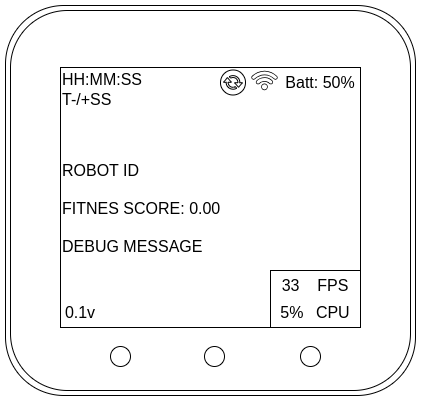
\includegraphics[width=0.35\textwidth]{UI.png}
    \caption{On-board debug/status display}
    \label{fig:UI}
\end{figure}

\end{document}